\documentclass[11pt]{article}

\usepackage{geometry}
\geometry{letterpaper, margin=0.64in}
\usepackage{censor}
\usepackage{dirtytalk}
\usepackage{xcolor}
\usepackage{amsmath}
\usepackage{hyperref}
\hypersetup{hidelinks,linkcolor = blue}
\usepackage{graphicx}
\usepackage{wrapfig}
\usepackage{fontspec}
\usepackage{listings}
\usepackage{xcolor}
\usepackage{wrapfig}

\definecolor{codegreen}{rgb}{0,0.5,0}
\definecolor{codegray}{rgb}{0.5,0.5,0.5}
\definecolor{codepurple}{rgb}{0.58,0,0.82}
\definecolor{backcolour}{rgb}{0.98,0.98,0.98}

\lstdefinestyle{mystyle}{
    backgroundcolor=\color{backcolour},   
    commentstyle=\color{codegreen},
    keywordstyle=\color{magenta},
%    numberstyle=\tiny\color{codegray},
    stringstyle=\color{codepurple},
%%    basicstyle=\ttfamily\footnotesize,
%    breakatwhitespace=false,         
%    breaklines=true,                 
%    captionpos=b,                    
%    keepspaces=true,                 
%%    numbers=left,                    
%    numbersep=5pt,                  
    showspaces=false,                
%    showstringspaces=false,
%    showtabs=false,                  
%    tabsize=2
}

\lstset{style=mystyle}


\begin{document}
\thispagestyle{empty}
\setlength\parindent{0pt}

\section*{CS50: Course notes}
\hrule
\vspace{0.25in}
CS50 is offered by Harvard University. I started this course in Aug 2020 on the edX platform. 

\noindent 
Course page: \href{https://cs50.harvard.edu/x/2020/}{https://cs50.harvard.edu/x/2020/}

\section*{Lecture 0: Computational thinking, Scratch}
Computer science at it's most basic level is problem solving. A typical workflow in CS takes an input and returns an output. Information in computers is stored in bits (1, 0). 8 bits are equivalent to 1 byte. 

\begin{itemize}
	\item $(11001)_2$ is equivalent to $1\times2^4 + 1\times 2^3 + 0\times2^2 + 0\times2^1 + 1\times 2^0 = (25)_{10}$
	\item Representing 50 in binary will require 7 bits, 110010
	\item Alphabets can also be represented in binary by creating a mapping. ASCII (American Standard Code for Information Interchange) was one of the first character encodings that used 8 bits to represent each alphabet, punctuation and digits. For example, `A' is represented with the binary equivalent of 65. Unicode is a much more flexible encoding that uses 1-4 bytes for encoding. As of Mar 2020, it supports 140k+ characters including emojis.
	\item Similarly, photos can be broken into pixel, and each pixel can be encoded as a tuple of 3 RGB values. Videos can be encoded as multiple pictures. Similarly, audio can also be digitally encoded taking into account pitch, note, volume, etc.
\end{itemize}

\subsection*{Phone directory search}
Let's say we want to search for a  particular name in the phone directory ($n$ pages), the brute force method of doing it is to go through each page from start to finish or until we find the name. In the worst case, we will need to visit $n$ pages before finding the name. A slight improvement will be to traverse 2 pages at a time. So, we start with page 2, then go to page 4, then page 6 and so on. If we happen to skip over the name, then we can go back to the previous page and search for it. With this approach, the worst case scenario will require visiting $n/2$ pages. 

We can extend this approach, and start at the middle of the phone book. Then based on the names on the page, we will either search it in the first half or the second. At each step we will keep splitting the search space by half. Via this approach, we will need to visit $\log_2(n)$ pages in the worst case. If the book at 1,024 pages. Then the first approach will require us to visit 1000 pages but with binary search approach, we need to only look at 10 pages. If the phone book size increased to 2048 pages, the binary search will only require us to look at just ONE additional page. 

\subsubsection*{Binary search algorithm for phone book}
\begin{enumerate}
	\item Open the book and go to the middle of the book
	\item If name found on the page: STOP
	\item Else if name is in the first half
	\item \begin{enumerate}
		\item Go to the middle of first half 
		\item Go to step 2
		\end{enumerate}
	\item Else if name if in the second half
	\item \begin{enumerate}
		\item Go to the middle of second half 
		\item Go to step 2 
		\end{enumerate}
	\item Quit as name is not found
\end{enumerate}

The key components of an algorithm are: a) functions, b) conditional statements, c) boolean expressions, d) loops, and e) variables. 

\subsection*{Homework}
The first homework was done using MIT's visual programming language called Scratch. It is accessible at this location: \href{https://scratch.mit.edu/}{https://scratch.mit.edu/}

\section*{Lecture 1: C}
The code that we write in a text-editor is called source code. Code written in C needs to be converted to machine code before it can be executed. To do this a compiler is needed. \texttt{clang} is an open-source compiler for C language. Executing the command \texttt{\$ clang program.c} creates a new executable file called \texttt{a.out} which stands for assembly output. This file is executable. 

This lecture showed the basic programming constructs in C like printing to screen, taking user input, data types, loops (for, do, while), conditional statements (if), boolean expressions, etc. Few notes: 
\begin{itemize}
	\item Do loop always executes once as it checks for the condition at the end of the first loop, whereas while loop checks the condition at the start. 
	\item Float precision\cite{floatingpoint}: in C takes up 4 bytes of space, and double takes 8 bytes. Float precision is the problem when 
	\item Numerical overflow: C stores datatype \texttt{int} with a storage size of 4-bytes. This will give it a range of $[-2^{31},\ 2^{31}]$. If we do a numeric operation on two \texttt{int} variables and the result exceeds this range, then we will run into numerical overflow. Such bugs may be hard to detect.
\end{itemize}

\subsection*{What happens during compilation}
When C code is compiled, it produces an executable file that contains machine code. The compilation step can be split into four main parts: 
\begin{enumerate}
	\item Preprocessing: In this step all the \texttt{\#include} statements are replaced by the corresponding lines from the header files. Header files contain references to functions declared in a library 
	\item Compiling: This step converts the source code into assembly language (machine code). This will typically have instructions that the CPU can understand. 
	\item Assembling: This step converts the assembly code into binary code (0s and 1s)
	\item Linking: If multiple files are involved in a source code, this step will merge the binary code from all files into a single executable file 
\end{enumerate}

\section*{Lecture 2: Arrays}
If we want to store a number of variables of the same type, using an \texttt{array} could make sense. For example, using an \texttt{array} to store the scores of a student from different subjects is a good idea. When declaring an \texttt{array} in C, we have to specify the size. 

\begin{lstlisting}[language=C]
// declaring an empty array of size 3
int scores[3];

// declaring an array of size 3 and initializing elements
int scores[3] = {100, 90, 85};
\end{lstlisting}

\subsection*{Strings}
\texttt{char} in C are implemented as mapping to 1-byte integers. For example, 'A' is mapped to 65. While \texttt{string} is not available by default, it can be implemented as an \texttt{array} of \texttt{char}. One peculiarity with strings is that they can be of arbitrary length. So, to signify the end of a string, we use a null character, $\backslash0$ which maps to a 1-byte integer of all zeros. So, a string 'EMMA' will take 5 bytes of memory. When an array of strings is initialized with with values 'EMMA', 'ADAM' and 'JOHNSON', the data structure will occupy 18 bytes of memory sequentially. 

\section*{Lecture 3: Algorithms}
The runtime complexity of an algorithm is typically measured via the Big-O ($\mathcal{O}$) notation. This represents the runtime order in the worst case scenario as a function of input size, $n$. As the value of $n$ gets larger, only the higher order terms are valid and hence in the big-O notation only the highest order term is retained. We can also define $\Omega$ as the complexity in best case scenario. Big-O complexity of a few common algorithms: 
\begin{enumerate}
	\item Linear search: $\mathcal{O}(n)$
	\item Binary search: $\mathcal{O}\left(\log(n)\right)$ (if the data is sorted)
	\item Bubble sort: $\mathcal{O}(n^2)$
	\item Selection sort: $\mathcal{O}(n^2)$
	\item Merge sort: $\mathcal{O}\left(n\log(n)\right)$ 
\end{enumerate}

\subsection*{Bubble sort}
\begin{wrapfigure}{r}{0.5\textwidth}
	\centering
	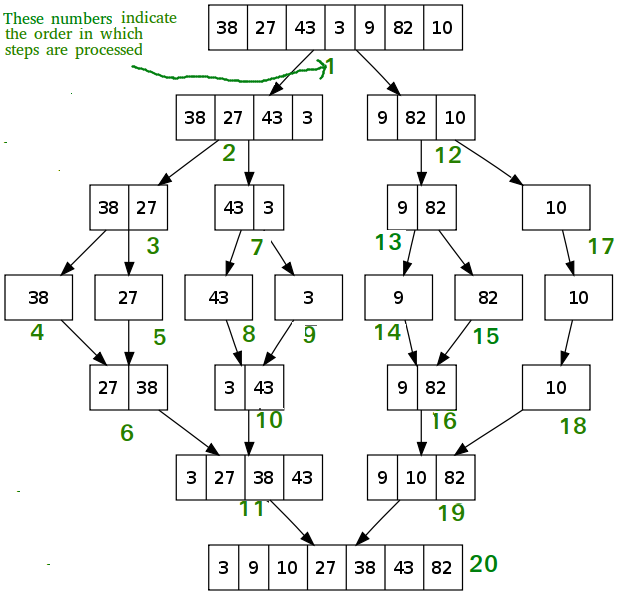
\includegraphics[width=0.9\linewidth]{figures/merge-sort}
	\caption{Merge sort example}
	\label{fig: merge-sort}
\end{wrapfigure}
We start by comparing the first two elements, if second element is smaller than the first, we swap the elements else we move to the next pair. This algorithm has the effect of bubbling the maximum value to the end of the list. We will need to do a total of $(n-1)$ passes. In the first pass, $(n-1)$ comparisons are needed, in the second pass, $(n-1)$ and so on. 



\subsection*{Selection sort}
In selection sort, we find the smallest value in each pass and swap it with the element in its sorted position. In the first pass, we run through the list and find the smallest element and then swap its position with the first element. In the second pass, we start with the second element and find the smallest element. We then swap its position with the second element. 

\subsection*{Merge sort}
Figure \ref{fig: merge-sort} explains the merge sort algorithm with an example. In merge sort, we split the list into two parts, then we sort each half independently using merge sort recursively. If the list has only one element, we return the element. Then we merge the two halves. Merging can be done in linear time. For a list of size $n$, we can do halves in $\log_2n$ steps. Hence, the runtime of merge sort is $\mathcal{O}\left(n\log(n)\right)$.

\section*{Lecture 4: Memory}
\begin{itemize}
	\item Computer memory can be thought of as divided into bytes. If a machine has 1GB of RAM, then there will be $\approx$1 billion bytes (exactly $2^{10}\times2^{10}\times2^{10}$ bytes). Each byte is allocated an address. This is often represented with a hexadecimal number prefixed by 0x. A byte in hexadecimal just needs two digits to be represented fully. For example 0xFF represents ($16^1\times15 + 10^0\times15=255$). That's why 24-bit colors can be represented as \#FF0000 (red). 
	\item Let's say we declare a variable in C as \texttt{int n = 0;}. The address of the variable can be found by using \texttt{\&n}. Similarly, if have a memory address stored in a variable, \texttt{p}, we can access the value stored at this address by using \texttt{*p}. The variable \texttt{p} is called the pointer as it points to another location in the memory. 
	\item \texttt{string} in C can be implemented as \texttt{char *s}. So, it is essentially a pointer to a location in memory. Each character is one byte long. So, string will contain all characters until the null character is encountered. For this reason, the string comparison using a comparison operator (\texttt{==}) doesn't work as is it comparing the memory addresses of two different locations. 
	\item Further, if we declare a string as \texttt{char *s = "EMMA"; char *t;} and then assign \texttt{t = s;}. Then we have assigned the memory address stored in \texttt{s} to \texttt{t}. The value \texttt{"EMMA"} has not been copied. As such, if we make a change to the value of \texttt{s}, \texttt{t} will also change. For copying strings, we must first allocate some space using \texttt{malloc} and then copy one character at a time ensuring that we also copy the null character. We should also remember to free up the allocated memory when done using it. We could also use the function \texttt{strcpy} from the \texttt{string.h} library. 
\end{itemize}

\begin{lstlisting}[language=C]
// declare an int
int n = 100;

// print the address of n
printf("%p\n", &n);

// declare a pointer to n
int *p = &n;

// print the address stored in pointer
printf("%p\n", p);

// print the value at address stored in pointer
printf("%i\n", *p);

// print the address of the pointer
printf("%p\n", &p);
\end{lstlisting}

\section*{Lecture 5: Data Structures}
\begin{itemize}
	\item The advantage of using arrays is that we can retrieve item at any index in constant time. Further, if the array is sorted then we can search for an item in $\mathcal{O}(\log(n))$ time. However, when using arrays, we have to declare the size of the array. If at a later point we need to add another element to the array, then we must allocate another location in memory, copy each element one at a time and then insert the new element. So, insertion in array requires linear time.
	\item An alternative way of storing a list of numbers is to use a linked list. Let's say we wanted to store 4 integers. Linked list will store these randomly across the available. But so that we are able to discover all numbers, we need an additional storage for each number to save a pointer to the next number in the list. Key advantage of a linked list is that we can insert new values without having to copy elements to a new location. However, we lose the ability to go to a particular index as easily as an array. For going to a particular index in a linked list, we have to traverse all preceding elements. So, this operation is $\mathcal{O}(n)$. 
	\item A hashtable is a mix of an array and a linked list. To store elements, a hashtable uses a hash function to choose the location in an array to put them at. For example, to store names in a hashtable, we could use the hash function as the first letter of the name. Egon can then be stored at index 4 in the hashtable and can be retrieved in constant time. Adding new elements can also be done in constant time. One drawback of the hashtables is they are prone to collisions. If we get a name like Erin, then we will not be able to store it at index 4 as the name Egon is already present there. So, we will need to build a linked list at index 4 with Egon as the first node and Erin as the second node. It is important to choose a hash function that can distribute the elements evenly across the array. 
	\item Trie uses a lot of memory but has the advantage that search and addition of new elements can be done in constant time. Trie is a linked list where each node is an array. In order to store names in a trie structure, we could store the first letter in an array of size 26. Then have a linked array to store the second letter and so on. 
	\item Binary search trees have the advantage that elements can be searched in $\mathcal{O}(\log(n))$. Key rule of binary search trees is that each node in the left sub-tree is smaller than the parent node, and each node in the right sub-tree is larger than the parent node. This allows searching for an element in $\mathcal{O}(\log(n))$. It is important to ensure that the tree remains balanced when adding or removing elements. 
\end{itemize}

\section*{Lecture 6: Python}
Unlike C, we don't have to compile Python code before running it. We use a program called \texttt{python} which can take command line arguments. If we pass the name of the program file, it will run the code. Python code gets compiled to machine language at the runtime. 	
\section*{Lecture 7: SQL}
If we want to look for a particular record in csv file, we will need to load the file in memory and then parse the file one record at a time. With csv files, we can only search in linear time. Databases have the advantage of improving on this. They implemented sophisticated data structures like B-tree to store indices which makes search for particular records much faster. 

\begin{enumerate}
	\item \texttt{sqlite} is a file based database that can be easily set up on any platform. Data can be loaded into it using either command line utility or a python program. 
	\item SQL injection attack: It is important to parse user input otherwise malicious actors could use it to delete information or login without proper credentials. When passing parameters to a SQL query in python, we shouldn't use f-strings. Instead, we should use question marks to pass parameters in the \texttt{db.execute} function. 
\end{enumerate}

\section*{Tracks: Web}
\begin{itemize}
	\item When devices communicate with each other on the internet, they send messages to each other. The sending and receipt of the messages follow established protocols. One such protocol is TCP/IP which stands for transmission control protocol/internet protocol. When we send letters in real world, we need to include the recipient and sender's addresses. Similarly, when sending messages over internet, we have to include the IP addresses of the recipient and sender. Further to differentiate between packets (webpages, email, file transfer, etc.), we include a port number in the recipient address. For example, port 21 is reserved for FTP, 25 is reserved for SMTP (emails).
	\item When we type an address like google.com in a web browser, a domain name system (DNS) will resolved that to an IP address. DNS servers maintain a mapping between the URL names and IP addresses. In a URL like http://example.com, the http part stands for hyper-text transfer protocol, which tells the recipient about the contents of the packets. 
\end{itemize}

\bibliographystyle{unsrt}
\bibliography{references}

\end{document}